

% The following makes latex use nicer postscript fonts.

\documentclass[a4paper,10pt]{report}

\usepackage[a4paper]{geometry}
\usepackage[dutch]{babel}
\usepackage{lmodern}
\usepackage{amssymb,amsmath}
\usepackage[T1]{fontenc}
%\usepackage[utf8]{inputenc}
\usepackage{microtype}
\usepackage{longtable,booktabs}
\usepackage[unicode=true]{hyperref}
\usepackage{graphicx}
\usepackage[space]{grffile}
\usepackage{lscape}
\usepackage{listings}
\usepackage{tabularx}
\usepackage{vubtitlepage}
\usepackage{tikz,pgfplots}
\usepackage{mathtools}
\usepackage{caption}
\usepackage{apacite}
\usepackage{subfig}
\usepackage{siunitx}
\usepackage{pgfplots} 
\usepackage{pgfplotstable}
\usepackage[round]{natbib}
\usepackage[toc,page]{appendix}
\usepackage{xr}
\usepackage{adjustbox}
\externaldocument{sections/lectuur}
\externaldocument{sections/experiment}
\newcommand{\argmax}[1]{\underset{#1}{\operatorname{arg}\,\operatorname{max}}\;}
\usepackage{array}
\usepackage{multirow}
\usepackage{tabu}

\newcommand\MyBox[2]{
  \fbox{\lower0.75cm
    \vbox to 1.7cm{\vfil
      \hbox to 1.7cm{\hfil\parbox{1.4cm}{#1\\#2}\hfil}
      \vfil}%
  }%
}
\setlength{\parindent}{0em}

\author{Yannick Merckx}
\title{Gevoelsanalyse in het Nederlands}

\promotortitle{Promotor}
\promotor{Yann-Micha\"el De Hauwere}
\advisors{Maarten Deville\\
          Peter Vrancx}
\advisortitle{Begeleiders}
\faculty{Faculteit Wetenschappen}
\department{Departement Computerwetenschappen}
\reason{Bachelorproef}
\date{Juni 2015}
\rolenumber{Rolnummer: 500294}
          
\begin{document}

% First dutch TitlePage
\maketitlepage

\setlength{\arrayrulewidth}{0.1mm}

\newpage

\begin{abstract}
Gevoelsanalyse is een populaire gegeven binnen de Machine Learning. In deze bachelorproef gaan we op zoek of het mogelijk is om aan de hand van enkele eenvoudige machine learning technieken een gevoelsanalyse uit te voeren. Specifieker focussen we op de Nederlandse taal, waar het naslagwerk vandaag de dag eerder beperkt van is. Als onderwerp van de gevoelsanalyse worden film-,boek- en muziekrecensies aan de hand van een algoritme beoordeeld of ze een positieve of negatieve emotie uitdrukken. Voor het onderzoek bekijken we de theoretische kant van een gevoelsanalyse, waar we de mogelijke technieken bespreken. Daarnaast wordt ook de praktische zijde uitgewerkt waar we de theoretische kennis gaan omzetten in een experiment. Dit experiment toont aan dat het mogelijk is om gevoelsanalyse uit te voeren op het Nederlands.
\end{abstract}

\renewcommand{\abstractname}{Dank woord}
\begin{abstract}
Het maken van een bachelorproef doe je nooit alleen, daarom ook een woord van dank aan enkele mensen waarop ik gedurende mijn eindwerkproces steeds kon terugvallen. Als eerste zou ik graag mijn begeleiders, Maarten Deville en Peter Vranckx, van harte willen bedanken voor hun grote steun en inzet gedurende het hele jaar. Ze waren gedurende het hele jaar altijd beschikbaar om op al mijn vragen een snel antwoord te geven. Als laatste wens ik ook mijn dank uit te drukken aan mijn promotor, Yann-Micha\"el De Hauwere. Bij de korte evaluaties was hij altijd aanwezig en stond hij mij altijd bij voor raad en daad.
\end{abstract}
\renewcommand{\contentsname}{Inhoud}
\tableofcontents
\include{sections/introductie}

\chapter{Lectuur}\label{Lectuur}

In dit hoofdstuk wordt de theoretische achtergrond besproken rond wat er juist gebeurd in hoofdstuk \ref{Experiment} tijdens het experiment. In \ref{Voorstelling dataset} bespreken we de voorstelling van de data voor het zelflerende algoritme. In \ref{Technieken voor Pre-Processing} bespreken we enkele optimalisatie technieken die kunnen helpen om de prestaties van het zelflerende algoritme te verbeteren. Daarna volgen in \ref{Leermethode} de zelflerende algoritmes zelf, waarin de werking van de algoritmes wordt uitgelegd. Als laatste volgt er in \ref{Bias en Variantie} meer informatie over bias en variantie, twee begrippen die van belang zijn om in acht te nemen tijdens het experiment.

\section{Voorstelling dataset}\label{Voorstelling dataset}
%
De voorstelling van de data is al een eerste element van  het experiment waarmee men rekening moet houden. We kunnen bijvoorbeeld rauwe data meegeven aan het zelflerend algoritme of we kunnen de tekst omvormen naar een vector die het aantal voorkomens van ieder woord in de tekst bevat. Voor het experiment kiezen we het tweede voorbeeld, waarbij we een document voorstellen als een vector met daarin de woordfrequentie.
In sectie \ref{Vector Space Methode} gaan we verder in op deze techniek, genaamd de vector space methode.

\subsection{Vector Space Methode}\label{Vector Space Methode}
%
De vector space methode is een methode waarbij we een document als een vector voorstellen waarbij ieder element overeenkomt met een woord en zijn frequentie in het document. De elementen van de vector worden ook wel features genoemd. Als men concreet een document voorstelt kan men zeggen dat document $j$ voorgesteld wordt door $d_{j}$ met $f_{ij}$ de frequentie van het woord $w_{i}$. Met de frequentie $f_{ij}$ bedoelt men het totaal aantal voorkomens van het woord $w_{i}$ in document $j$. Het aantal verschillende woorden in het document stelt men voor door $n_{w}$, wat eveneens de dimensie is van de vector.
Het document $j$ kan dus als volgt worden voorgesteld:
%
\[ d_{j}  = \begin{bmatrix}
    f_{1j} \\
    f_{2j} \\
    \vdots \\
    f_{n_{w}j} \\
\end{bmatrix}  
\]
%
Een belangrijk inzicht bij de vector space methode is dat een document voorgesteld wordt als een groep van woorden. Er wordt geen rekening gehouden met de volgorde waarin de woorden in het document voorkomen. Vaak ziet men ook dat de vector vaak ijl is en vanwege de grote hoeveelheid aan woorden in een document heel groot. Als we nu niet \'e\'en document, maar meerdere documenten nemen en we zeggen dat het aantal documenten gelijk is aan $n_{d}$, resulteert dit in een matrix waarbij iedere kolom een document voorstelt.
\[
D =
 \stackrel{\mbox{Documenten}}{%
    \begin{bmatrix}
    f_{11} & f_{12} & \cdots & f_{1n_{d}} \\
    f_{21} & f_{22} & \cdots & f_{2n_{d}} \\
    \vdots & \vdots & \ddots & \vdots \\
    f_{n_{w}j} & f_{n_{w}2} & \cdots & f_{n_{w}n_{d}}
    \end{bmatrix}
    }
    & Woorden \]
%
Deze matrix wordt een \textbf{\textit{terms-documents matrix (TDM)}} genoemd. Wanneer men spreekt van een \textbf{\textit{documents-terms matrix (DTM)}}, spreekt men een getransponeerde terms-documents matrix. Een rij van een DTM stelt dan een document voor. In het experiment stellen we onze data voor aan de hand van een documents-terms matrix
%
De voorstelling in een matrix geeft inzicht en biedt veel meer mogelijkheden om de data te analyseren. We kunnen bijvoorbeeld al eenvoudig een afleiding maken over het verband tussen documenten.
Door de euclidische afstand te bepalen tussen twee rijen in de DTM kunnen we al zien of de documenten gelijkaardig zijn of niet. Stel men heeft twee documenten met een kleine euclidische afstand. Dit wil zeggen dat de vectorvoorstelling van de documenten gelijkaardig is, wat neerkomt op overeenkomstige woordfrequenties en dus bijvoorbeeld over hetzelfde onderwerp gaan of eenzelfde mening uitdrukken.
%
In de praktijk is gebleken dat documenten vergelijken op basis van woordfrequentie niet altijd de gewenste resultaten oplevert. Vaak is het nog altijd moeilijk om verschillend groepen tussen de documenten te onderscheiden. Daarom kan men nog extra verfijningen toepassen zoals bijvoorbeeld \textbf{\textit{term weighting}} of \textbf{\textit{Latent Semantic Analysis (LSA)}}.


\section{Technieken voor Pre-Processing}\label{Technieken voor Pre-Processing}

Zoals we in \ref{Vector Space Methode}  al zeiden bestaan er nog verfijning die we kunnen toepassen op de documents-terms matrix. Het verfijnen wordt ook wel de pre-processing of voorverwerking van de dataset genoemd en kan op verschillende manieren gebeuren. Men kan bepaalde data filteren zoals in \ref{Verwijderen van stopwoorden en leestekens} waar men stopwoorden en leestekens uit de dataset verwijdert. Men kan ook het DTM analyseren en en een nieuwe weging van de features introduceren zoals bijvoorbeeld bij term weighting of LSA gebeurd. Het doel van de pre-processing is de data zo goed mogelijk voor te bereiden zodanig dat het zelflerende algoritme een duidelijk beeld kan krijgen over hoe en naar wat het de inkomende data moet classificeren.

\subsection{Bag of Words}\label{Bag of Words}

Bag of Words is de eenvoudigste methode die er is en is het principe waarop de vector space methode zich baseert. Ieder document wordt beschouwd als een zak met woorden, waarbij de woorden in het document de kenmerken of de features van het document voorstellen. Bag of Words wordt beschouwd als de eenvoudigste techniek, omdat men bij de techniek geen rekening houdt met spelling, woordorde of voorkomens. Dit gaat wel het geval zijn bij andere technieken.

\subsection{Verwijderen van stopwoorden}\label{Verwijderen van stopwoorden en leestekens}

Wat men vaak ziet in het Nederlands, maar ook in taal algemeen, is dat er veel stopwoorden worden gebruikt. Stopwoorden als ``klopt'' en ``eigenlijk'' zeggen niet veel over teksten of ze nu positief of negatief zijn. Als een bepaald woord niet bijdraagt voor het algoritme kunnen we stopwoorden beschouwen als ruis in de dataset. Ruis vertroebelt het beeld van het concept dat we het algoritme willen aanleren en proberen we te elimineren. Daarom beschouwt men het verwijderen van stopwoorden en leestekens ook als een manier van pre-processing.

\subsection{Term weighting}\label{Term weighting}

Als we terugkijken naar de vector space methode, waarbij we enkel rekening houden met de woordfrequentie, kan men zeggen dat niet elk woord evenveel doorweegt. Een woord dat in alle documenten voorkomt biedt geen of minder waardevolle informatie, dan een woord dat zelden voorkomt. En hierop baseert term weighting zich. Het gaat een wegingsfactor introduceren. Ieder woord krijgt een gewicht toegewezen, dat weergeeft hoe belangrijk het woord is. Neem als voorbeeld een hoop recensies van de film ``Pulp Fiction'' en de woorden ``Pulp'' en ``excellent''. ``Pulp'' is een woord dat voorkomt in de titel van de film en komt ongetwijfeld in elke recensie voor. ``Excellent'' daarentegen is een woord dat enkel maar voorkomt wanneer de recensist de film fantastisch vond, het zal niet in elk document voorkomen en is waardevolle informatie. Term weighting zal dus bij dit voorbeeld ``excellent'' een groter gewicht toewijzen dan ``Pulp''. 
%
De kwantiteit van dit gewicht wordt vaak de \textbf{inverse document frequency  (idf)} genoemd en wordt bepaald aan de hand van volgende formule:
\[w_{i}: idf_{i} = -log_{2}[P(w_{i})] \]
met $P(w_{i})$ de priori probability dat woord $w_{i}$ voorkomt in het document.\\
%
De inverse document frequency geeft het algemeen belang van het woord $w_{i}$ weer. Men kan dit benaderen door het logaritme te nemen van het aantal documenten waar $w_{i}$ in voorkomt en het totaal aantal documenten.
Een andere nuttige kwantiteit is de  \textbf{term frequency} $tf_{ij}$. Deze geeft het belang weer van het woord $w_{i}$ binnen in het document $d_{j}$  en wordt als volgt genoteerd:
\[ tf_{ij} = \frac{f_{ij}}{ \sum_{i=1}^{n_{w}}f_{ij}} \]
%
$tf_{ij}$ wordt berekend door de frequentie, het aantal voorkomens, van een woord $w_{i}$ in document $d_{j}$ te delen door de som van alle woordfrequenties in document $d_{j}$.
Met deze twee kwantiteiten kan men een nieuwe begrip introduceren: de \textbf{tf-idf score}. Wat overeenkomt met het product van tf en idf.
\[ \text{tf-idf score} = tf . idf_{ij} = idf_{i} . tf_{ij} \]
%
De tf-idf matrix bekomt men dan door alle woordfrequenties van het terms-document matrix te vervangen door de tf-idf score.
Deze matrix wordt bijvoorbeeld vaak gebruikt om de gelijkenissen tussen twee documenten te bepalen op basis van cosinusgelijkenis.


\subsection{Bigram Collocaties}\label{Bigram Collocaties}

Bigrams Collocaties is een techniek waarbij men op zoek gaat naar paren van woorden die een hoge waarschijnlijkheid hebben om samen voor te komen en een extra bron van informatie kunnen vormen. De bepaling van de informatieve waarde van de bigrams is gebaseerd op de frequentie van het bigram en de frequenties van de andere bigrams. Als men een overzicht krijgt over de frequenties introduceert men een metriek, die met behulp van de frequenties mogelijke verbanden kan blootleggen. Chi-kwadraat is zo'n metriek die er zich toe leent. De Chi-kwadraattoets is een statistische toets die het mogelijk maakt om de onafhankelijkheid tussen waarnemingen te onderzoeken. Bij Bigram Collocaties onderzoekt men via de Chi-kwadraattoets de afhankelijkheid tussen twee woorden. Hoe grotere de afhankelijkheid, hoe hoger de score.   

\subsubsection{Chi-Kwadraattoets}\label{Chi-Kwadraattoest}

De Chi-Kwadraattoets is een techniek uit de statistiek die gebruikt  kan worden als een onafhankelijkheidstoets voor waarnemingen. De reden waarom we deze toets voor Bigram collocatie gebruiken is dat de toest parametervrij is. Wat wil zeggen dat er bij de start van de chi-kwadraattoets geen aanname over de populatie of het gemiddelde wordt verwacht. In deze sectie leggen we aan de hand van een voorbeeld uit hoe de chi-kwadraattoets juist deze afhankelijkheid bepaald.\\
%
Neem als voorbeeld het bigram \textit{(heel , goed)}. Zoals bij iedere statistische test neemt men eerst een nulhypothese aan. Voor de chi-kwadraattoets is dit ook het geval. De toets neemt als nulhypothese aan dat beide woorden onafhankelijk van elkaar zijn en elkaars voorkomen niet be\"invloeden. Men vergelijkt de waargenomen frequenties van de woorden met de verwachte frequenties wanneer de woorden onafhankelijk zouden zijn. Als deze waarden te veel verschillen kan men de nulhypothese verwerpen en de alternative hypothese aannemen, namelijk dat de woorden afhankelijk zijn van elkaar. \\
\newline
%
Om de afhankelijkheid van woorden te bepalen, kijken we naar volgende gegevens:
\begin{itemize}
  \item het aantal voorkomens van het woord in een bigram
  \item het aantal voorkomens van het woord in een bigram met het ander woord waar we de afhankelijkheid van onderzoeken
  \item het totaal aantal bigrams
  \item het aantal voorkomens van het ander woord in een bigram. 
\end{itemize}
%
%
Als we voor het voorbeeld \textit{(heel , goed)} bovenstaande gegevens in een kruistabel gieten krijgen we de volgende 2x2 tabel:
\begin{table}[h!]
\centering
\begin{tabular}{|l|c|r|}
\hline
          & w1= heel                                                         & w1 ≠ heel                                                                \\ \hline
w2 = goed & \begin{tabular}[c]{@{}c@{}}9\\ (heel goed)\end{tabular}          & \begin{tabular}[c]{@{}r@{}}7893\\ (bv. niet goed)\end{tabular}           \\ \hline
w2 ≠ goed & \begin{tabular}[c]{@{}c@{}}3632\\ (bv. heel slecht)\end{tabular} & \begin{tabular}[c]{@{}r@{}}13498000\\ (bv. boeiende thesis)\end{tabular} \\ \hline
\end{tabular}
\end{table}
\newline
We weten nu naar wat we moeten kijken bij het analyseren van de afhankelijkheid maar er mist nog een weging, een onderlinge verhouding tussen de kenmerken. 
%
De Chi-Kwadraatsom biedt hier de oplossingen en geeft die weging. De toetsingsgrootheid voor de Chi-kwadraattoets wordt gedefinieerd aan de hand van de volgende formule:

\[{\chi}^2=\sum_{i,j}^{} \frac{(O_ij - E_ij)^2}{E_ij}\]
%
Waarbij ${O_ij}$ het aantal keer dat het paar $(i,j)$ voorkomt. $E_ij$ stelt de voorspelde waarden voor als de woorden onafhankelijk moesten voorkomen\\
$E_ij$ wordt bepaald door volgende formule:

\[{E_ij}= \frac{O_i*}{N} + \frac{O_*j}{N} * N = \frac{O_i* O_*j}{N} \]
%
met $\frac{O_i*}{N}$ de marginale probabiliteit dat $i$ als eerste deel van het bigram voorkomt en $\frac{O_j*}{N}$ de marginale probabilitiet dat $j$ als tweede deel van het bigram voorkomt. $N$ stelt het totaal aantal bigrams voor.
%
Toegepast op het voorbeeld geeft dit voor het bigram ``(heel , goed)'':

\[{E_11} = \frac{9+3632}{N}+\frac{9+7893}{N} * N \approx 0,0085 \]
\newline
Als laatste onderdeel berekenen we de ${\chi}^2$-score, bepalen we het aantal vrijheidsgraden en zoeken we de ${\chi}^2$ distributie op met de berekende vrijheidsgraad. Stel dat het vooropgestelde betrouwbaardheidsinterval 95\% bedraagt dan kunnen we de kritische waarde bepalen voor significantielevel $\alpha$ = 0,005.
Als de berekende ${\chi}^2$-score in het verwerpingsgebied ligt, kan de nulhypothese verworpen worden en kan het bigram beschouwd worden als afhankelijk.\\
%
Onderstaande afbeelding illustreert hoe de verwerping of aanvaarding van een nulhypothese juist in zijn werking gaat
%
\begin{figure}[h]%
    \centering
    \subfloat{{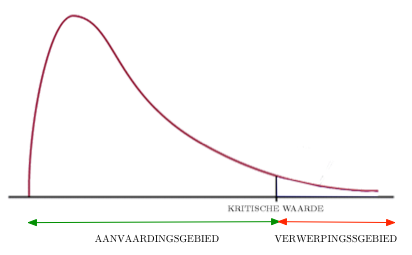
\includegraphics[width=10cm]{confidence_interval_chi_square} }}%
    \caption{Illustratie eenzijdige-toets van een ${\chi}^2$-distributie [Orginele afbeelding: http://www.philender.com/courses/intro/notes3/xdist.gif]}%
\end{figure}
\newline
Kort samengevat baseert de Chi-kwadraattoets zich op de afwijking tussen de geobserveerde frequentie en de verwachte frequentie. Hoe groter het verschil, hoe waarschijnlijker men de nulhypothese kan verwerpen. En dit is waar men zich bij Bigram Collocatie op gaat baseren.

\begin{figure}[h]%
    \centering
    \subfloat{{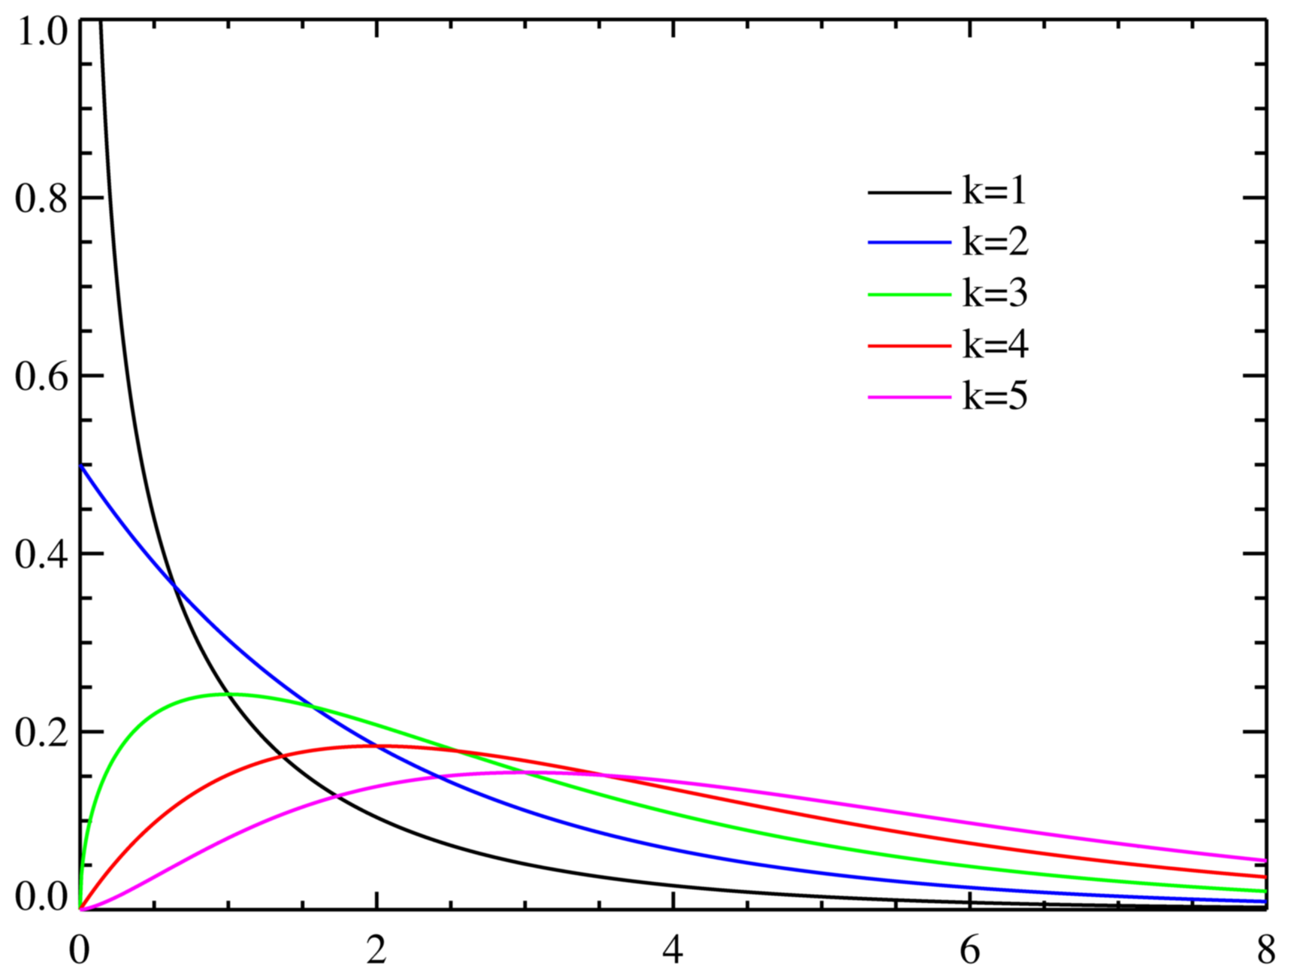
\includegraphics[width=6cm]{Chi-square_distribution} }}%
    \caption{Chi-square distributies met K vrijheidsgraden [Bron: \url{http://upload.wikimedia.org/wikipedia/commons/2/21/Chi-square_distributionPDF.png}]}%
\end{figure}

\subsection{Best feature selection}\label{Low-information feature el}

Als we duizenden documenten verwerken, is het te voorspellen dat er enorm veel woorden algemeen voorkomen in de documenten, maar niet veel informatie bijdragen over het document zelf. Het is sterk vergelijkbaar met de voorgaande techniek in \ref{Verwijderen van stopwoorden en leestekens} bij het verwijderen van stopwoorden. Veel voorkomende features kunnen voor het document niet als iets identificerend dienen en zorgen voor ruis in de dataset. Daarom kan men verkiezen om deze low-information features te verwijderen zodanig dat men enkel de features overhoudt die echt iets zeggen over een document. Het bepalen van de informatiewinst kan gebeuren aan de hand van het aantal voorkomens in de verschillende klassen. Als een bepaalde feature voornamelijk in positieve documenten voorkomt en amper in negatieve documenten, kan men afleiden dat deze feature zeer informatief is omtrent positieve documenten. Als metriek om de informatiewinst te meten kan men wederom ${\chi}^2$ uit \ref{Chi-Kwadraattoest} gebruiken. Chi-kwadraat laat ons namelijk toe om de correlatie tussen een bepaalde feature en de klassen te meten.
%
\subsection{Latent Semantic Analysis}\label{Latent Semantic Analysis}

Latent Semantic Analysis is een wiskundige techniek gebaseerd op statistische berekeningen. Met LSA probeert men een notie te krijgen van de semantische informatie en meer bepaald het semantisch verband tussen woorden. Bijvoorbeeld als we zoeken naar documenten met het woord ``economie'', willen we ook documenten met ``financi\"en'' terugkrijgen. Voor LSA zijn twee woorden semantisch gerelateerd als ze gebruikt worden in dezelfde context. Met het concrete voorbeeld kunnen we zeggen dat er een semantisch verband is tussen twee woorden als ze vaak voorkomen in dezelfde documenten.
\newline
Merk op dat bij Latent Semantic Analysis het belangrijk is dat ieder woord naar \'e\'en concept verwijst.
%
\newline
Analytisch wordt LSA toegepast door \textbf{Singular Value Decomposition (SVD)} toe te passen op de terms-documents matrix. SVD is een concept uit de lineaire algebra en zegt dat een matrix A opgesplitst kan worden als een product van matrixen namelijk \\
\[A = U\Sigma V^T \]
De reductie van de dimensie gebeurt aan de hand van volgend principe
%
%afbeelding van SVD in latex
\newcommand{\vect}{\mathbf}
\newcommand{\nul}{\operatorname{Nul}}
\newcommand{\col}{\operatorname{Kolommen }}
\newcommand{\row}{\operatorname{Rijen}}
\[
   A= U\Sigma V^T=
  \begin{matrix}
    \underbrace{\left[\begin{matrix}\vect u_1 & \vect u_2 & \dots & \vect u_r\end{matrix}\right.}& 
    \underbrace{\left.\begin{matrix}\vect u_{r+1} & \dots &  \vect u_m\end{matrix}\right]}\\
    \col A & \nul A^T
  \end{matrix}
  \begin{bmatrix}
      \sigma_1 & 0 & \dots & 0 & 0 & \dots & 0 \\
         0 & \sigma_2  & \dots & 0 & 0 & \dots & 0 \\
         \dots& & & & &  \\
         0 & 0 & \dots & \sigma_k  & 0 & \dots & 0 \\
         0 & 0 & \dots & 0 & 0 & \dots & 0 \\
         \dots& & & & &  \\
         0 & 0 & \dots & 0 & 0 & \dots & 0 
  \end{bmatrix}
  \begin{bmatrix}
    \vect v_1^T \\ \vect v_2^T \\ \dots \\ \vect v_r^T \\
    \vect v_{r+1}^T \\ \dots \\ \vect v_n^T
  \end{bmatrix}
  \begin{matrix}
    \left.\vphantom{\begin{bmatrix}
       \vect v_1^T \\ \vect v_2^T \\ \dots \\ \vect v_r^T 
       \end{bmatrix}}\right\}\row A \\ 
    \left.\vphantom{\begin{bmatrix}
      \vect v_{r+1}^T \\ \dots \\ \vect v_n^T 
    \end{bmatrix}}\right\}\nul A
  \end{matrix}
\] 
\newline
U is de unitaire matrix waarbij men $u_1, u_2, ... , u_n$ de linker singuliere vectors noemt. Deze stellen een document met zijn features voor. $V^T$ is de geconjugeerde getransponeerde matrix van V. $v_1, v_2, ... , v_n$ noemt men de rechter singuliere vectors en stellen de woorden met hun features over alle documenten voor. $\Sigma$ is een diagonaal matrix met singuliere waarden $\sigma_1,\sigma_2,..,\sigma_n$'  op de diagonaal. De reductie van een terms-documents matrix naar een dimensie van $K$ gebeurt door de hoogste $K$ singuliere waarden te nemen in $\Sigma$ met de overeenkomstige singuliere vectoren uit $U$ en $V$.    
Doordat men de dimensionaliteit van de vectoren kan beperken door semantisch gelijkaardige woorden bijeen te voegen. Laat dit toe om een soort van context groepen te cre\"eren en zo een zeker inzicht te krijgen in de dataset. Het is dan ook gebleken dat SVD toepassen een zeer nuttige eerste stap is bij text mining \cite{maas2011learning}, omdat men nieuwe meer effici\"ente features krijgt. De nieuwe features geven meer duidelijkheid en inzicht en kunnen dienen als input voor het zelflerende algoritme.

\section{Leermethode}\label{Leermethode}

Zoals we al zeiden in de introductie, gaan we beroep doen voor het experiment op technieken uit de Machine Learning. Specifieker gaan we voor het experiment gebruik maken van supervised learning technieken.
Dit is een subdomein binnen de Machine Learning waarbij we het algoritme trainen met een dataset die voorbeelden bevat over het concept dat we willen aanleren. De trainingsset bevat zowel de inputwaarden als de verwachte outputwaarde voor de input en men verwacht dat het zelflerende algoritme hier verbanden in kan vinden zodanig dat het voor willekeurige inputwaarden de juiste outputwaarde kan bepalen. Voor het experiment tekst als input, classificeren als positief of negatief. In de Machine Learning noemt men dit probleem een classificatieprobleem. Dit is een probleem waarbij inputwaarden, in het experiment de recensies, geclassificeerd moeten worden naar een kleine set van mogelijkheden. In het geval van het experiment bestaat die set van mogelijkheden uit positief en negatief.\\
%
Nu we het experiment gesitueerd hebben als een classificatieprobleem dat men gaat oplossen met technieken of algoritmes uit supervised learning, kunnen we deze algoritmes eens bekijken.\\  
%
Wanneer we een zelflerende algoritme iets proberen aan te leren, tracht het algoritme een hypothese of model te vormen waarmee het de output kan voorspellen. Het algoritme is een bepaalde leermethode, die het mogelijk maakt om verbanden af te leiden uit de trainingsset en zo een hypothese op te stellen.
Er zijn veel leermethodes \cite{mitchell1997machine}, maar we bespreken enkel de relevante leermethode tot het experiment namelijk Naive Bayes Learning en Decision Tree Learning. In \ref{Naive Bayes Classifier} en \ref{Decision Tree} bespreken we de werking van deze methodes en bekijken we de eigenschappen, wat ze zo passend maakt voor het experiment.  

\subsection{Naive Bayes Classifier}\label{Naive Bayes Classifier}

Als eerste leermethode hebben we de Naive Bayes Classifier. Deze is gebaseerd op Bayesiaans redeneren. Bayesiaans redeneren is een aanpak die gevolgen trekt op basis van probabiliteit. Het is gebaseerd op de veronderstelling dat bepaalde hoeveelheden die ons interesseren probabilistisch verdeeld zijn en door te redeneren over die probabiliteit samen met de trainingsdata er optimale beslissingen kunnen genomen worden.\\%
Naive Bayes is een van de praktische aanpakken naar bepaalde leerproblemen \cite{mitchell1997machine}. In een studie \cite{Michie94machinelearning} rond Naive bayes classifiers werd de  prestatie ten op zichte van andere leeralgoritmen, zoals beslissingsbomen en neurale netwerken onderzocht. Hierin werd aangetoond dat de Naive Bayes Classifier gelijkaardig presteert als de andere leermethode en in sommige gevallen zelfs beter.\\
%
De werking van de Naive Bayes Classifier is volledig gebaseerd op probabiliteit. Neem als inputwaarden $x_{1} , x_{2}, x_{3}, ..., x_{n}$ en als de te voorspellen outputwaarde $y_{res}$. Nu moet de classifier voor de inputwaarden $x_{1} , x_{2}, x_{3}, ..., x_{n}$ de correct $y_{res}$ voorspellen. Volgens het Bayesiaans redenering is, gebaseerd op $x_{1} , x_{2}, x_{3}, ..., x_{n}$,  $y_{res}$ de outputwaarde met de grootste waarschijnlijkheid. We kunnen dit neerschrijven als:

\[y_{res} = \underset{y_i \in Y}{\arg\max}P(y_i|x_{1},x_{2},x_{3},...,x_{n}) \] 

Aan de hand van het Bayes theorema kunnen we dit herschrijven als

\[ y_{res} = \underset{y_i \in Y}{\arg\max}\frac{P(x_{1},x_{2},x_{3},...,x_{n}|y_i)P(y_i)}{P(x_{1},x_{2}, x_{3},...,x_{n})} \]

 Merk op $P(x_{1},x_{2},x_{3},...,x_{n})$ is gelijk aan 1, aangezien dit gegeven is dus

 \[ y_{res} = \underset{y_i \in Y}{\arg\max}P(x_{1},x_{2},x_{3},...,x_{n}|y_i)P(y_i) \]
%
 De twee componenten kunnen bepaald worden aan de hand van de trainingsset. $P(y_i)$ kunnen we bepalen door het aantal voorkomens van $y_i$ in de trainingsset te tellen. $P(x_{1},x_{2},x_{3},...,x_{n}|y_i)$ is moeilijker af te leiden aan de hand van de trainingsset aangezien we meerdere voorkomens van $x_{1},x_{2},x_{3},...,x_{n}$ naar $y_i$ moeten hebben om een goede schatting te kunnen maken.  Indien we een heel grote trainingsset hebben is dit mogelijk, anders niet. Om dit toch te kunnen afleiden, gaat de Naive Bayes Classifier er van uit dat elke $x_i$ uit $x_{1},x_{2},x_{3},...,x_{n}$ onafhankelijk is ten opzichte van de outputwaarde $y_i$. Wat betekend dat we het product van iedere probabiliteit kunnen nemen en $P(x_{1},x_{2},x_{3},...,x_{n}|y_i)$  kunnen herschrijven als $\prod\limits_{i} P(x_{i}|y_{i})$.\\
%
Samengevat is de Naive Bayes Classifier een goede eerste keuze als leermethode aangezien zijn goede algemene prestatie \cite{Michie94machinelearning}. Voor het maken van voorspelling maakt het gebruik van probabiliteit, gebaseerde op de trainingsset en waar het aanneemt dat ieder feature onafhankelijk is tot de outputwaarde. Samengevat kunnen we dit schrijven als

 \[y_{NBres} = \underset{y_i \in Y}{\arg\max} P(x_{i})\prod\limits_{i} P(x_{i}|y_{i}) \]
%
Ten slotte stellen we de verzameling van al deze probabiliteiten samen als de hypothese van de Naive Bayes Classifier.

\subsection{Decision Tree}\label{Decision Tree}
%
Als tweede leermethode hebben we de Decision tree of beslissingsboom. Beslissingsbomen is een van de meest gebruikte en praktische methode voor inductieve gevolgtrekking \cite{mitchell1997machine}. De methode is robust met ruis op de data en kan om met discrete klassen. De techniek gaat een beslissingsboom proberen op te stellen aan de hand van de trainingsdata. Na de training krijgt men dan een beslissingsboom die de hypothese moet voorstellen. Wanneer het getrainde algoritme onbekende data krijgt, gaat het inductief de output bepalen voor de inputwaarden. Men kan een beslissingsboom voorstellen als een disjuncte set van als-dan regels.\\ 
%
Onderstaande afbeelding is een voorbeeld van zo'n beslissingsboom die bepaald of het weer goed genoeg is om basketbal buiten te spelen. De bladeren van de boom stellen de verschillende outputwaarden voor. In dit geval zien we dat er een boom is opgesteld voor twee discrete klassen namelijk ja en nee. In de nodes staan testen beschreven die de het pad van de inputwaarden naar de outputwaarde bepalen. Merk op dat de bepaling altijd top-down gebeurd.
%
\begin{center}
  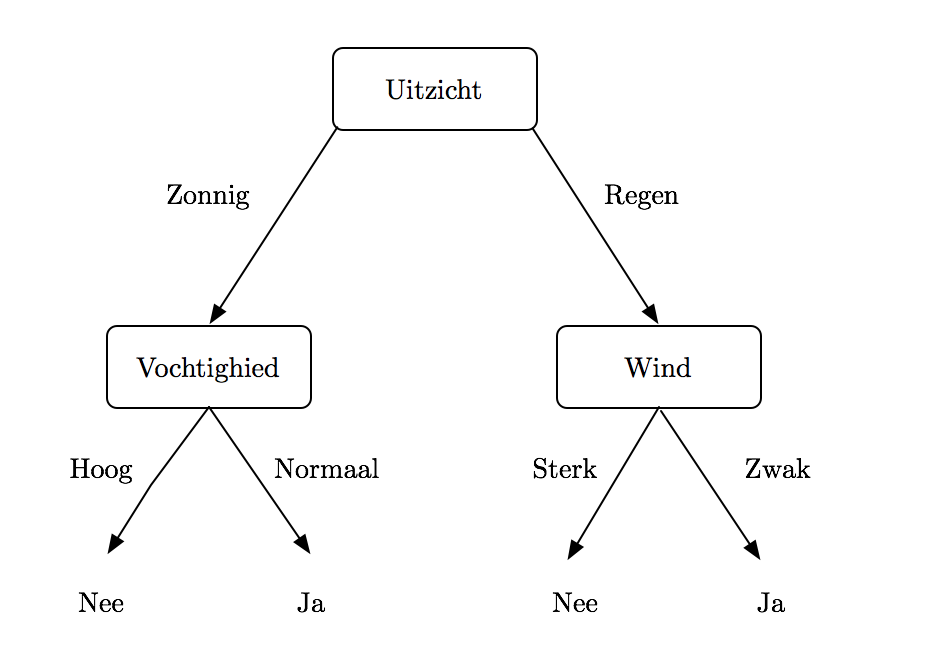
\includegraphics[width=10cm]{decisiontree}
  \captionof{figure}{Voorbeeld van een beslissingsboom}
  \label{fig:beslissingsboom}
\end{center}
%
In het algemeen zijn beslissingsbomen het best gepast voor problemen met volgende kenmerken \cite{mitchell1997machine}: 

\begin{itemize}
  \item{Inputwaarden worden voorgesteld door attribuut-waardeparen.}
  \item{Zowel de trainingsdata als de testdata mag errros bevatten}
  \item{Sommige elementen van de trainingsset mogen attributen missen}
\end{itemize}

Al deze characteristieken zijn gunstig voor het experiment. In \ref{Voorstelling dataset} zagen we dat de data kan voorgesteld worden door de vector space methode. Een document kunnen we hier beschouwen als input met de woorden en hun aantal voorkomens als het de attribuut-waardeparen. Verder is het bij het verzamelen van data nooit uitgesloten dat de data errors bevat en moet de classifier hier bestand tegen zijn.

\section{Bias en Variantie}\label{Bias en Variantie}

Wanneer we bepaalde modellen onderzoeken is het belangrijk om te weten waarom een bepaald model niet goed presteert. De slechte prestatie kan door verschillende redenen worden veroorzaakt \cite{mitchell1997machine}. Twee mogelijke oorzaken zijn modellen met een hoge bias en een hoge variantie.\\
%
%
Wanneer we een model trainen zoals bijvoorbeeld een Decision tree uit \ref{Decision Tree}, stelt het model aan de hand van de trainingsdata een hypothese op en aan de hand van de hypothese gaat het model dan voorspelling maken over de ongekende data. Als we nu meermaal een nieuwe analyse uitvoeren met telkens een nieuw model met een andere trainingsset, maar over hetzelfde concept en we bekijken voor elk getraind model de voorspelling voor telkens dezelfde testset. Dan meet Bias hoe ver in het algemeen de getrainde modellen hun voorspelling afwijken van de correcte waarden. Wanneer de voorspellingen sterk afwijken van de correcte waarden, spreekt men van hoge bias.  De variantie duidt op de spreiding van de voorspellingen. Wanneer er een groot verschil is tussen de voorspellingen van de modellen voor een bepaald punt, en dit is gemiddeld ook zo voor de andere punten, dan spreekt men van een hoge variantie.\\
%
Onderstaande afbeelding geeft een grafische weergave hoe variantie en bias zich tegenover elkaar verhouden en wat voor invloed het heeft.
De afbeelding stelt een bulls-eye diagram voor waarbij de gele punten de hypotheses van de getrainde modellen voorstellen. Hoe dichter de gele punten bij het centrum van de roos liggen, hoe beter en correcter de voorspellingen. Wanneer de trainingsdata bijvoorbeeld goed verdeeld is, gaan de gele punten dicht bij de roos liggen. Wat duidt op een lage variantie en lage bias. In tegenstelling tot wanneer de dataset vol met outliers en afwijkende waarden gaat zitten. De punten gaan dan heel verspreid en ver van de roos liggen. Wat duidt op een hoge variantie en hoge bias.\\
%
\begin{center}
  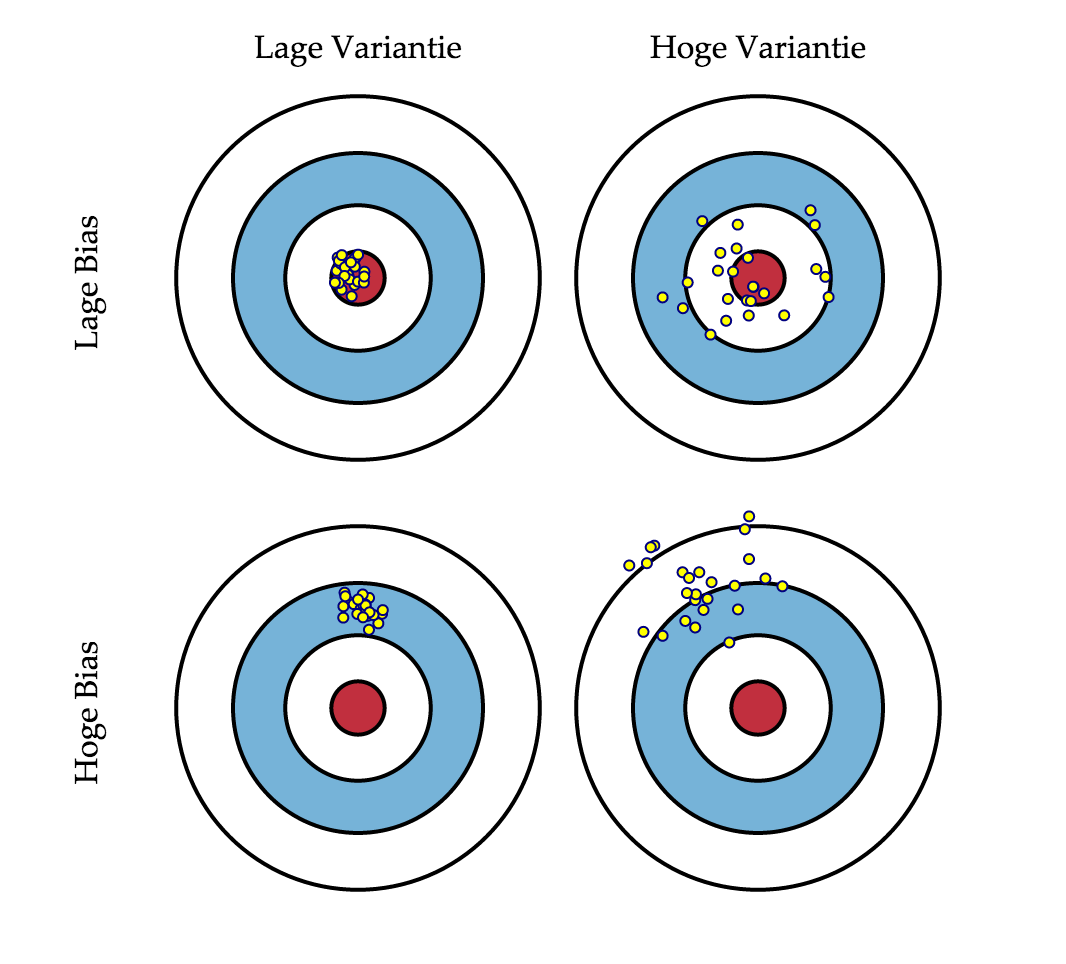
\includegraphics[width=10cm]{bulls-eye}
  \captionof{figure}{Schematische weergave van Bias en Variantie (Gebaseerd op:\url{http://scott.fortmann-roe.com/docs/BiasVariance.html})}
\end{center}
\newline
Concreet kan men zeggen wanneer men te maken heeft met bias en variantie, dat men werkelijk te maken heeft met over- en underfitting. Men spreekt van overfitting wanneer de resultaten op de trainingsset goed zijn, maar voor onbekende sets veel minder.\\
Stel dat we ons model steeds uitbreiden door het te blijven trainen. Als resultaat stijgt de complexiteit van ons model, wat maakt dat het beter voorspellingen kan doen, dus de bias vermindert, maar er gaan meer outliers en afwijkende waarden zijn. En dus de variantie stijgt. Wat dus maakt dat er een trade-off is tussen bias en variantie.\\ 
%
Wiskundig kunnen we dit ook aantonen. Neem $Y$ als de variable de we willen voorspellen en $X$ als de variable die de inputwaarden voorstelt. Neem ook dat er een relatie bestaat tussen de twee $Y=f(X)$. We willen nu door het algoritme te trainen met de inputwaarden, een hypothese $f_{p}(X)$ maken voor $f(X)$. \\
Neem nu dat we $f(X)$ willen voorspellen door lineaire regressie te gebruiken en de hypothese te beoordelen aan de hand van de squared prediction error. Dit is een metriek om de kwaliteit van de hypothese te bepalen. Hoe hoger de kwaliteit van het model, hoe lager de squared prediction error van het model. Als we nu de formule van squared prediction error er bij nemen:

\[ Err(X)=E[(Y - f_{p}(X))^2] \]
%
met $E$ de verwachtingswaarde.\\
%
Als we deze formule nu herschrijven in functie van bias en variance componenten \cite{hastie2009elements}, krijgen we :

\[ Err(X)=(E[f_{p}(X)] - f(X))^2+E[f_{p}(X) - E[f_{p}(X)]]^2 \]
%
Wat neerkomt op 

\[Err(X)= Bias^2 + Variantie \]
%
Hier zien we wederom dat er een keuze moeten maken tussen het minimalisatie van bias en de minimalisatie van variantie.
Onderstaande afbeelding illustreert nogmaals het verband tussen bias en variantie en hoe deze zich bijdraagt tot de totale error.
\begin{center}
  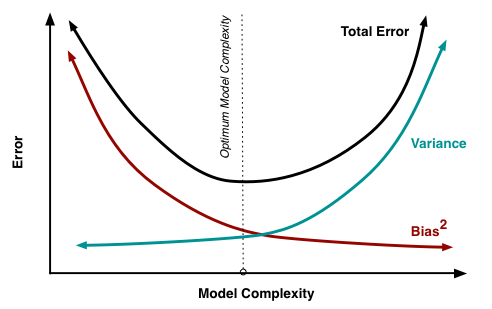
\includegraphics[width=10cm]{biasvariance_tradeoff}
  \captionof{figure}{Bijdrage Bias en Variantie aan totale error (Bron:\url{http://scott.fortmann-roe.com/docs/docs/BiasVariance/biasvariance.png})}
  \label{fig:biasvariance}
\end{center}
\newline
Zoals men kan zien op bovenstaande afbeelding is het optimum voor de complexiteit van het model, de plaats waar de totaal error het laagste is. Als we nog preciser kijken zien we dat dit de plaats is waar de bias evenveel vermindert als de variantie toeneemt. Wiskundig kunnen we dit formuleren als volgt:

\[\frac{dBias}{dComplexiteit} = -\frac{dVariantie}{dComplexiteit} \]
%
In de praktijk is er spijtig genoeg geen analytische methode om dit punt te vinden en moet men samen met de squared predict error functie experimenteren met verschillende levels van complexiteit voor een model en hier het level van complextiteit met de laagste totale error uit selecteren.\\
%
Nu dat we een goed algemeen begrip hebben over bias en variantie, kijken iets dieper in op over- en underfitting.

\subsubsection{Over- en Underfitting}\label{Over- en Underfitting}

Eerder zeiden we al wanneer men spreekt of bias en variance, men eigelijk bezig is met over- en underfitting. Laten we eerst nog eens kijken wat juist overfitting is. \citet{mitchell1997machine} definieert overfitting als volgt:
\newline
\newline
\textit{Given a hypothesis space H , a hypothesis h E H is said to overfit the training data if there exists some alternative hypothesis h' E H, such that h has smaller error than h' over the training examples, but h' has a smaller error than h over the entire distribution of instances.}
\newline
\newline
Wat eigenlijk wil zeggen dat hypothese H te goed werkt op zijn eigen trainingsset, maar vanaf het andere waarden begint te classificeren is de prestatie veel minder. Bij underfitting is het juist omgekeerd. De prestatie is lager op de trainingsset dan op een grote nieuwe dataset. Het te goed presteren van een trainingsset, wil eigelijk zeggen dat het model te precies, te complex is afgesteld. Aan de hand van figuur \ref{fig:biasvariance}, kunnen we afleiden dat dit duidt op een hoge variantie. Gelijkaardig met underfitting, wanneer het getrainde model slecht presteert met zijn eigen trainingsset, wil dit zeggen dat het model te eenvoudig, niet complex genoeg is. Wat duidt op een hoge bias (zie figuur \ref{fig:biasvariance}).
%
Het verband nog eens kort samengevat. Wanneer men spreekt van underfitting, spreekt men van hoge bias. Wanneer men spreekt van overfitting, spreekt men van hoge variantie.

\begingroup
\section{Latent Semantic Analysis (LSA) Experiment}\label{Latent Semantic Analysis Experiment (LSA) Experiment}

We stellen nu een proefopstelling op en we gaan het de vector space methode bij text mining toepassen op een echt voorbeeld.

\subsection{Proefopstelling}\label{Proefopstelling}
Als eerste verkrijgen we onze trainingsset door de polarity v2 dataset (website: http://www.cs.cornell.edu/People/pabo/movie-review-data) te downloaden. Deze dataset bevat positieve en negatieve recensies van imdb. We hebben te maken met supervised learning, want we weten welke recensies positief en welke negatief zijn. Het doel van het experiment is door middel van de geziene technieken zoals de vector space methode met latent semantic analysis en term weighting een inzicht te krijgen in de dataset en we proberen gelijkaardige recensies te groeperen. Tenslotte onderzoeken we de hypothese, waarbij we zeggen hoe meer features we hebben voor een document, hoe groter de nauwkeurigheid bij de classificatie.


\subsection{Werkwijze}\label{Werkwijze}

De werkwijze verloopt als volgt.
Eerst passen we document pre-processing toe. We halen alle stopwoorden en leestekens uit de dataset. Vervolgens stellen we een document-term matrix op. Dan optimaliseren we deze matrix voor classficatie door de matrix om te vormen naar een tf-idf matrix. Dit is de techniek waarbij we iedere frequentie $f_{ij}$ van een woord $w_{i}$ vervangen door de tf-idf score van het woord. Daaropvolgend reduceren we de dimensie van onze tf-idf matrix naar twee door de latent semantic methode toe te passen. Iedere recensie wordt na de reductie voorgesteld door middel van twee features. 
De recensies plotten we dan met elke recensie als een punt met een andere kleur voor positieve en negatieve recensies.
Ten slotte nemen we terug onze tf-idf matrix en reduceren het naar door een bepaald aantal features bijvoorbeeld 10, 50, 100, 500. En we kijken of onze hypothese geld waarbij we betere classificatie resultaten krijgen bij meer features.

\subsection{Resultaten}\label{Resultaten}

Als resultaat zien we dat het invoeren van term weighting zoals de tf-idf matrix echt wel nut heeft voor dat we de latent semantic methode toepassen.
Als we de twee plots vergelijken, de ene zonder term weighting dan andere met term weighting, zien we duidelijk dat we bij diegene met term weighting duidelijk twee groepen kunnen onderscheiden.

\begin{figure}%
    \centering
    \subfloat[LSA zonder term weighting]{{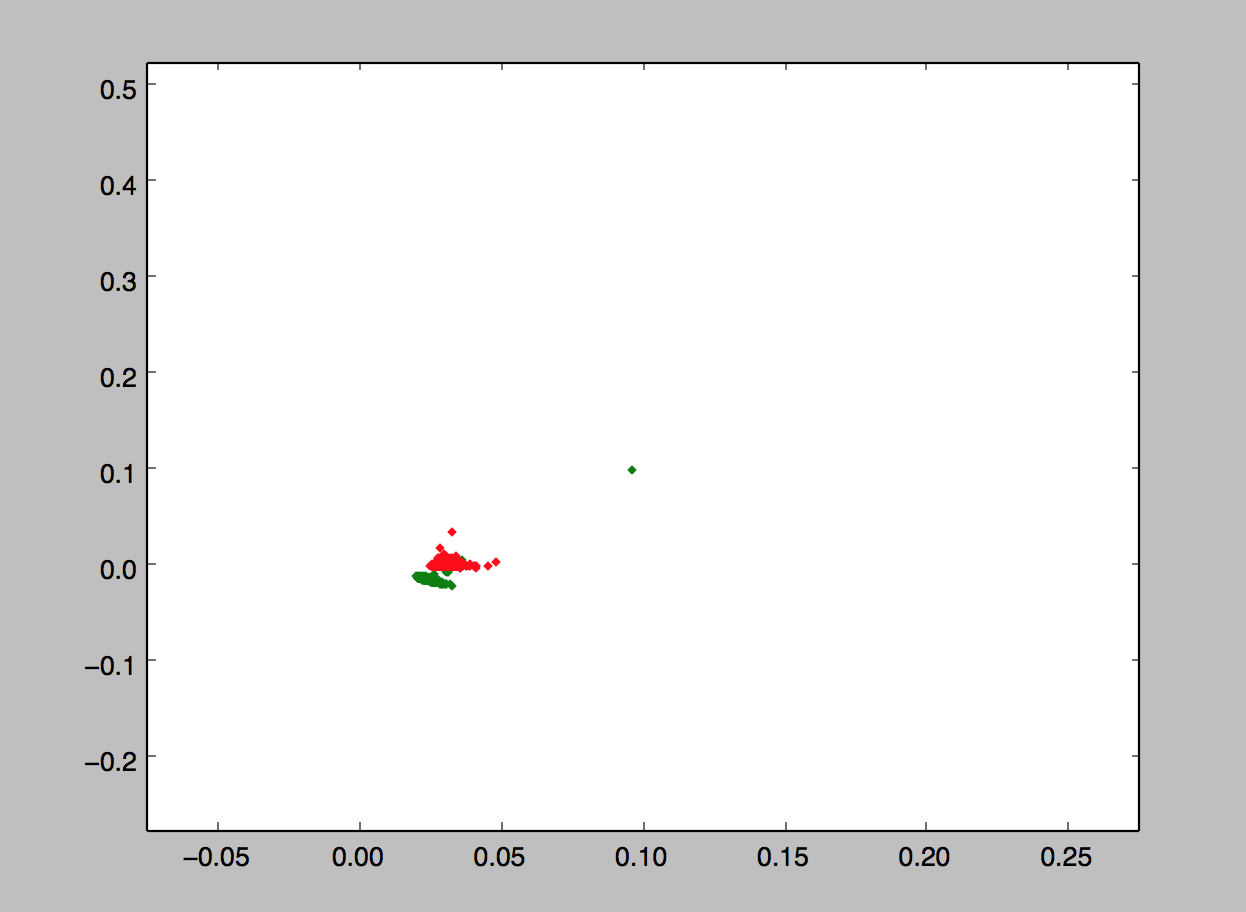
\includegraphics[width=5cm]{experiment_1} }}%
    \qquad
    \subfloat[LSA met term weighting]{{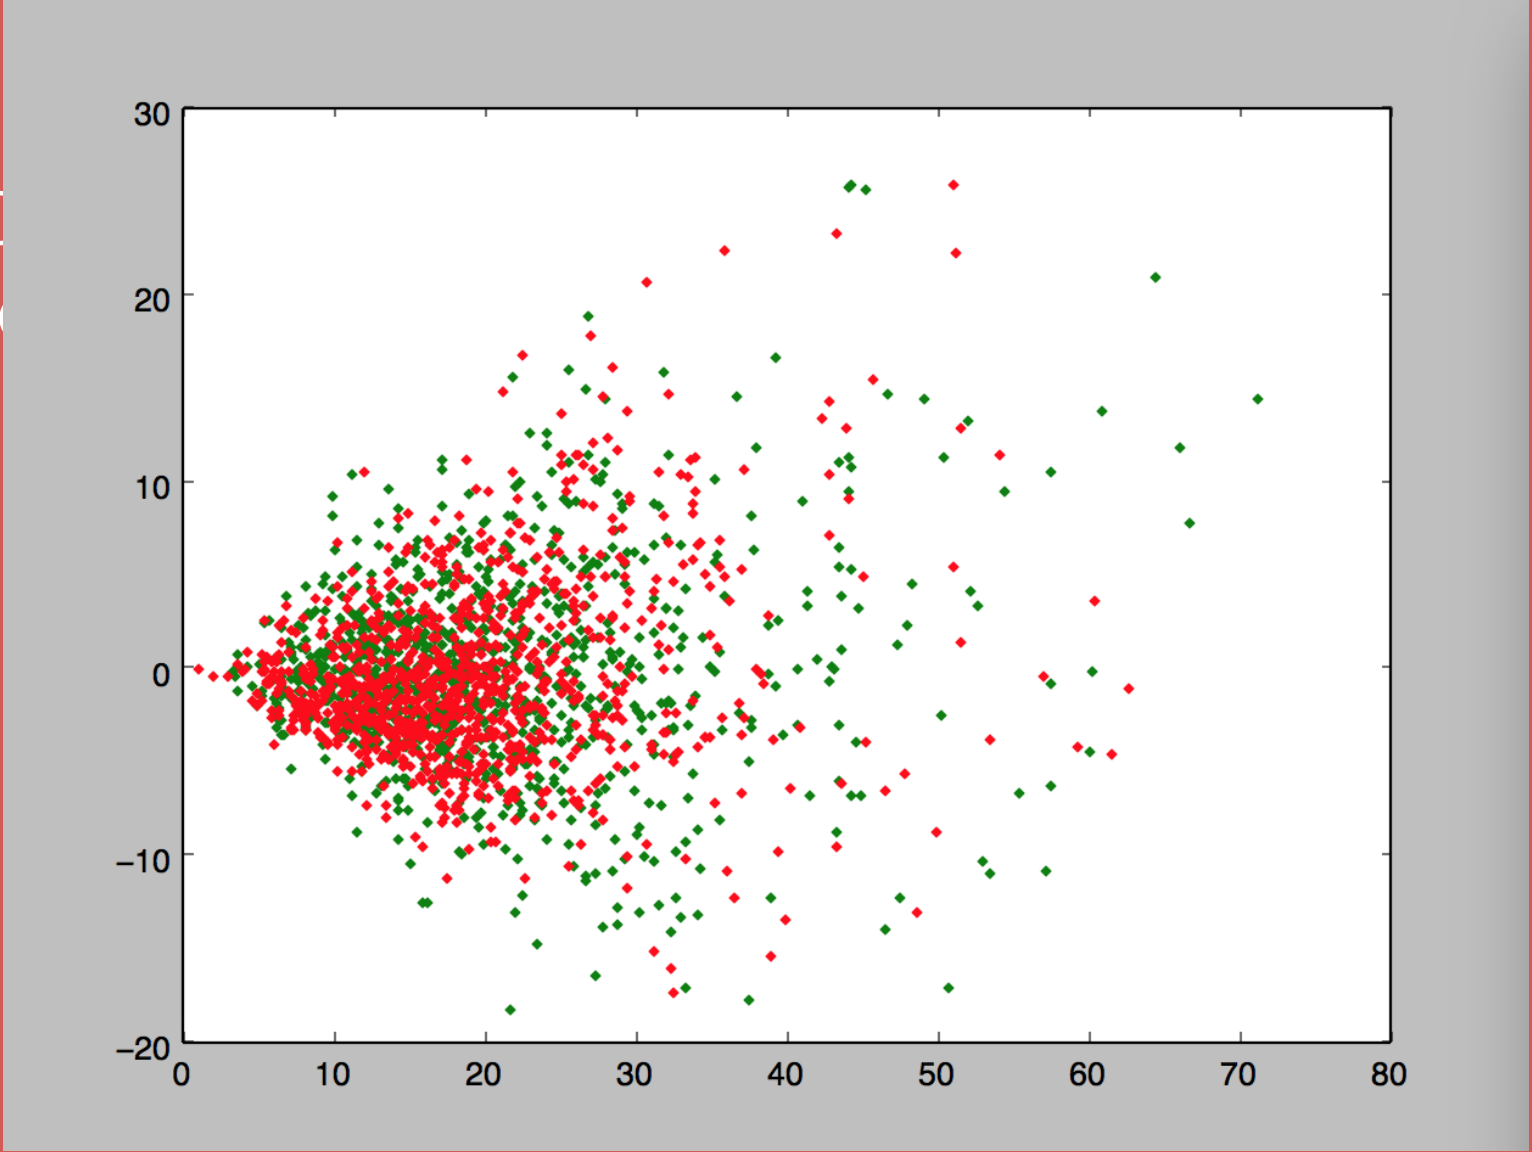
\includegraphics[width=5cm]{experiment_2} }}%
    \caption{Effect van term weighting voor LSA}%
    \label{fig:example}%
\end{figure}
%
Tenslotte kunnen we ook onze hypothese bevestigen. We zien dat de hoeveelheid aan features, de nauwkeurigheid van de classificatie beïnvloed. Onderstaande afbeelding geeft deze relatie weer. De x-waarde stelt het aantal gelijkaardige recensies dat men opvraagt voor. De y-waarde geeft aan hoeveel er gemiddeld effectief juist geclassifiseerd zijn. Belangrijk om te weten is dat de dataset voor de helft uit positieve recensies bestaat en voor de helft uit negatieve. We trachten dus bij de classificatie een gemiddeld percentage van 50 percent te halen en we zien dat op onderstaand voorbeeld de lijn van 500 features hier het beste in slaagt.


\begin{center}
  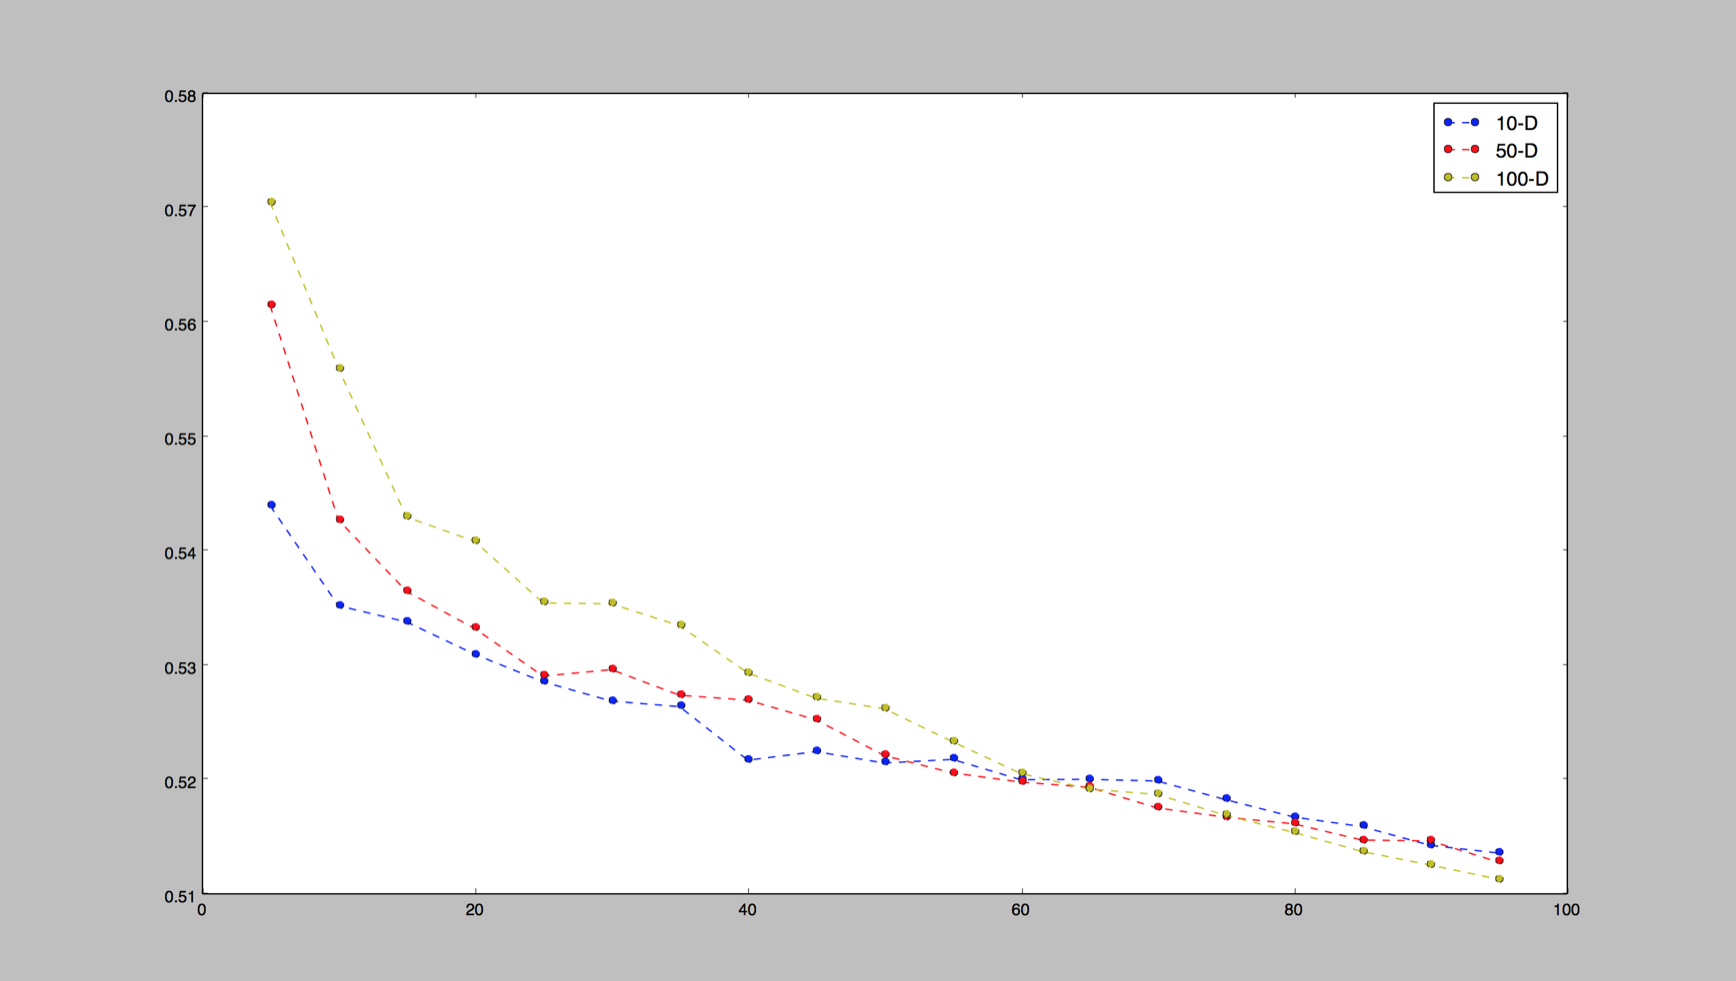
\includegraphics[width=10cm]{experiment_3}
  \captionof{figure}{Nauwkeurigheid van de classificatie bij een verschillend aantal features}
\end{center}
\endgroup
\chapter{Conclusie}\label{Conclusie}

Voor deze bachelorproef gingen we onderzoeken of de werkwijzen voor engelstalige gevoelsanalyse ook toepasbaar zijn voor nederlandstalige gevoelsanalyse en proberen we deze verschillen beter te specificeren. We hebben getracht om aan de hand van een experimentele analyse hier een antwoord op te vinden.
In de experimentele analyse hebben we een algemeen beeld proberen te vormen over Nederlandse gevoelsanalyse. We hebben in \ref{Engelse gevoelsanalyse versus Nederlandse Gevoelsanalyse} een directe vergelijking gemaakt met Engelse gevoelsanalyse. In deze vergelijking zagen we dat Engelse gevoelsanalyse in het algemeen beter presteerde dan Nederlandse gevoelsanalyse, maar dat voor beide gevoelsanalyses er goede resultaten werden behaald. En de technieken voor Engelse gevoelsanalyse wel degelijk overdraagbaar zijn naar Nederlandse gevoelsanalyse. We zijn mogelijke oorzaken van die betere prestatie voor het Engels gaan onderzoeken. Hieruit konden we besluiten dat de impact van de hoeveelheid woorden (data) in een tekst een rol spelen in de prestatie. We zagen een duidelijk prestatie voordeel bij de Engelse dataset met langere woorden. Dit bevestigd nogmaals dat een goed presterende gevoelsanalyse met de huidige technieken enkel mogelijk is voor meer substanti\"ele teksten, en moeilijk tot onmogelijk voor kortere stukken tekst.\\
Ook zagen we in beide analyseresultaten dezelfde trends. Zo zagen we voor beide talen de Naive Bayes Classifier in combinatie met het verwijderen van stopwoorden, Term weighting en Bigrams als beste techniek en zagen we dezelfde prestatieverschillen tussen de algoritmen mee overgaan van het Engels naar het Nederlands.\\

Vervolgens hebben we classificatie onderzocht op basis van geannoteerde woordenlijsten van gevoelens. Hier hadden we voor de Nederlandse woordenlijsten, een vertaling gebruikt van de Engelse woordenlijsten. Hier konden we besluiten dat Engels woordenlijsten niet transparant vertaald kunnen worden naar het Nederlands en de classificatie onvoldoende presteert. We zagen hier deels de oorzaak lag bij een andere woordenschat, leenwoorden, schrijffouten, internetslang en uitgesmeerde woorden. In verder onderzoek kan men deels deze invloeden wegnemen door de woordenlijsten zelf samen te stellen op basis van een Nederlandse dataset en hier de prestatie van te onderzoeken. Een andere opvallende bevinding uit dit experiment is de opvallende overeenkomst van negatieve engelstalige woorden in onze Nederlandse dataset. Dit kan ook een gevolg zijn van de herkomst van onze Nederlandse dataset (een ‘internetpubliek’ dat onder andere veel gebruikt maakt van anglicismen).\\

Als laatste hebben we de invloed van jargon onderzocht bij Nederlandse gevoelsanalyse. Hier zagen we dat wanneer men een classifier traint voor een bepaald jargon deze ook het beste presteert voor dat jargon. Ook zagen we dat een algemeen concept, het onderscheiden van een positieve en negatieve opinie, kan aangenomen worden door de classifier, desondanks het jargon in de datasets.\\

We hebben aangetoond dat technieken voor gevoelsanalyse grotendeels overdraagbaar zijn, al is het belangrijk om rekening te houden met het feit dat technieken die afhangen van uitgebreid geannoteerde woordenlijsten vaak niet rechtstreeks te vertalen zijn. Voor deze aanpakken is het dus nodig om per taal aangepaste woordenlijsten op te stellen. Maar gezien de goede prestaties van technieken die zonder deze lijsten kunnen werken, kunnen we stellen dat het vaak interessanter is om te investeren in de ontwikkeling van een goede herbruikbare leertechniek in plaats van een uitgebreide geannoteerde woordenlijst per taal.
\newpage
\nocite{*}
\bibliographystyle{apacite}
\bibliography{sections/Thesisbib}
\end{document}
    
    
        